\documentclass[../diploma.tex]{subfiles}
 
\begin{document}

	\label{sec:experiments}
	
	Для оценки качества различных модификаций было произведено тестирование обученных нейронных сетей на тестовой выборке.
	
	\subsection{Используемые метрики}

	Для сравнения моделей использовалось несколько метрик, классических для задачи бинарной классификации:

	\begin{itemize}

	    \item
		Аккуратность: 
		\begin{equation}
			Acc = \frac{TP + TN}{TP + FP + FN + TN}
   		\end{equation}

	    \item
		Точность: 
		\begin{equation}
			P = \frac{TP}{TP + FP}
   		\end{equation}

	    \item
	    Полнота: 
		\begin{equation}
			R = \frac{TP}{TP + FN}
   		\end{equation}

	    \item
		$F$-мера, позволяющая объединить точность и полноту в единую метрику:
        \begin{equation}
			F_1 = \frac{2 \cdot P \cdot R}{P + R}
   		\end{equation}

	    \item
	    Площадь под $ROC$-кривой ($AUC$)~--- графиком, показывающим зависимость количества верно классифицированных положительных примеров 
	    от количества неверно классифицированных отрицательных примеров при изменении порога решающего правила.
		
	\end{itemize}

	В упомянутых выше формулах использованы следующие обозначения:

	\begin{itemize}

		\item
		$TP$~--- количество верно классифицированных правильных ответов.

		\item
		$FP$~--- количество неверно классифицированных правильных ответов.

		\item
		$FN$~--- количество неверно классифицированных неправильных ответов.

		\item
		$TN$~--- количество верно классифицированных неправильных ответов.
	\end{itemize}

	\subsection{Производительность}

	Обучение и тестирование производилось на GPU Tesla V100 с $16$ гигабайтами памяти.
	Обучение одной модели занимало несколько часов (от $4$ в случае сверточной сети до $15$ в случае рекуррентной).

	\subsection{Результаты}
		
	Было произведено тестирование и сравнение моделей, описанных в разделе \ref{sec:methods}, 
	с показателями исследований, упоминавшихся в подразделе \ref{subsec:existing_solutions},
	а также с двумя наивными алгоритмами:

	\begin{itemize}
	
		\item
		Наивный байесовский классификатор, на вход которому подается векторное представление ответа по модели Bag of Words с мерой \texttt{TF-IDF}.
		Для тестирования использовалась реализация из фреймворка Scikit-Learn \cite{online:scikit_learn}.

	    \item
	    Классификатор, который считает правильным ответ, который был дан раньше остальных.

	\end{itemize}

	\vskip 1em
	\begin{table}[ht]
		\centering
        %\small
        \begin{tabularx}{\textwidth}{| l | X | l | l | l | l | l |}
	        \hline
    	    \textbf{Модель} & \textbf{Виды признаков} & $\mathbf{Acc}$ & $\mathbf{P}$ & $\mathbf{R}$ & $\mathbf{F_1}$ & $\mathbf{AUC}$ \\ \hline
	        \hline
    	    First-answer & метаинформация & 0.66 & 0.69 & 0.60 & 0.64 & 0.66 \\ \hline
        	Naive-Bayes with TF-IDF & словарные & 0.6 & 0.58 & 0.54 & 0.56 & 0.59 \\ \hline
	        \hline
    	    Burel et al. \cite{article:burel2012} & лингвистические, словарные, пользовательские, метаинформация & - & 0.77 & 0.77 & 0.76 & 0.83 \\ \hline
        	Tian et al. \cite{article:tian2013} & лингвистические, метаинформация & 0.72 & - & - & - & - \\ \hline
	        Gkotsis et al. \cite{article:gkotsis2014} & лингвистические, словарные, метаинформация & - & 0.83 & 0.66 & 0.74 & 0.85 \\ \hline
    	    \hline
	        FC & лингвистические, словарные, метаинформация & ? & ? & ? & ? & ? \\ \hline
	        CNN & текстовые, лингвистические, словарные, метаинформация & \textbf{0.77} & 0.81 & 0.62 & 0.71 & \textbf{0.86} \\ \hline
    	    RNN & текстовые, лингвистические, словарные, метаинформация & \textbf{0.78} & 0.82 & 0.64 & 0.72 & \textbf{0.87} \\ \hline
        \end{tabularx}
		\caption{Сравнения качества работы различных моделей}
		\label{tab:results}
	\end{table}

    Был произведен перебор таких параметров модели, как размерность выхода \texttt{LSTM}-ячеек в рекуррентной архитектуре или количество фильтров в сверточной, 
    а также коэффициент Dropout и размер скрытого слоя, и выбраны в качестве используемых в итоге те, которые показывают лучшие результаты на проверочной выборке.

    Результаты сравнения приведены в таблице \ref{tab:results}.

	\subsection{Анализ результатов}

	\label{subsec:results}

	Как мы видим из таблицы, лучше всего себя показала модель, 
	использующая двунаправленную рекуррентную архитектуру и функцию $AESD$ для анализа сходства текстов вопроса и ответа.

	На рисунке \ref{fig:roc} представлена \texttt{ROC}-кривая, соответствующая этой модели, 
	из которой, в частности, видно, что благодаря метаинформации 
	наш классификатор выдает высокие оценки вероятности в большинстве своем правильным ответам (кривая смещена влево).

	\vskip 1em
    \begin{figure}[ht]
   	    \centering
		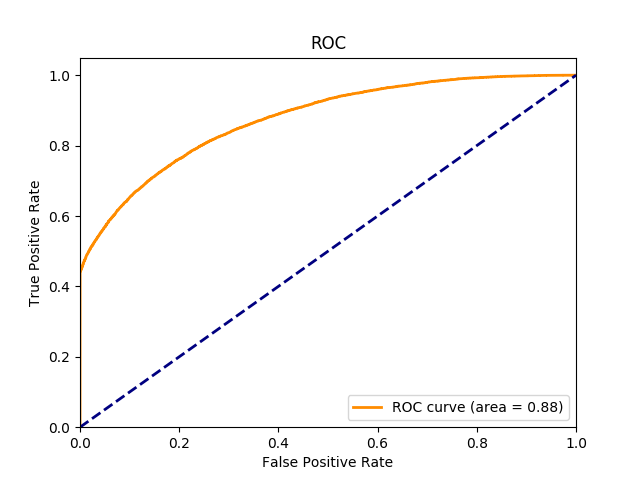
\includegraphics[width=0.9\linewidth]{images/roc.png}
   		\captionof{figure}{\texttt{ROC}-кривая}
		\label{fig:roc}
   	\end{figure}

	Анализируя полученные результаты, можно отметить следующие вещи:

	\begin{itemize}
	
		\item
		Результаты модели, не использующей семантическое представление вопроса совпадают с результатами модели, 
		которая использует только лингвистические и словарные признаки, а также метаинформацию.
		То есть векторное представление текста ответа в отрыве от вопроса не помогает определить, насколько ответ хорош.
		В целом, это ожидаемый результат, ведь подобная векторизация создана для передачи смысла текста, что неприменимо в дальнейшем без текста вопроса.

		\item
		Были протестированы модели, обучающие параметры сверточных либо рекуррентных слоев и совместно для вопросов и ответов, и по отдельности.

		Оказалось, что архитектура с совместными параметрами, во-первых, быстрее обучается, а во-вторых, 
		показывает лучшие результаты на проверочной выборке.
		Это сходится с показателями других работ по тематике выбора ответа, например \cite{article:answer_selection}.

		\item
		Были протестированы модели, использующие различные функции определения похожести вопроса и ответа.

		При использовании функций конкатенации и суммы время обучения увеличилось по сравнению с тремя остальными, 
		кроме того, они давали худшие результаты при тестировании на проверочной выборке.

		Несмотря на то, что в работе \cite{article:answer_selection} функция $AESD$ показывала более хорошие результаты,
		в нашем случае все три остальные функции (косинусный коэффициент, $GESD$ и $AESD$) давали в среднем одинаковые метрики.

		\item
		В целом, использование текстовых признаков дало незначительный прирост по сравнению с моделью, которая использует признаки остальных типов.
		Вероятно, это связано с тем, что большая часть вопросов в датасете ожидает описание некоторого процесса, 
		а не какой-то короткий фактологический ответ.
		Кроме того, даже для человека поставленная задача не является простой: 
		только в $87 \%$ случаев ответ с максимальным рейтингом (рейтинг рассчитывается с помощью оценок других пользователей) отмечается автором вопроса как наилучший.

		Тем не менее, реализованная модель превосходит как базовые алгоритмы, так и уже существующие решения, использующие другие методы машинного обучения, 
		по метрикам аккуратности и площади под $ROC$-кривой, которые наиболее полно описывают качество бинарного классификатора.
	\end{itemize}


\end{document}

